\documentclass{article}
\usepackage[utf8]{inputenc}
\usepackage{graphicx}
\usepackage{wrapfig}
\usepackage{siunitx}
\usepackage{amssymb}
\title{STUDY OF NETWORK THEOREMS\\KIRCHHOFF'S CURRENT/VOLTAGE LAW}
\author{Aditya Agrawal\\2021AM10198\\GROUP 29}
\date{April 15, 2022}

\begin{document}

\maketitle
\tableofcontents
\newpage
\section{Kirchhoff's Laws}
\subsection{Aim}
To verify Kirchhoff's laws of Current and Voltage in a circuit.

\subsection{Apparatus}
\begin{enumerate}
    \item Multiple Power Supply
    \item Resistors (1 of 47 Ω, 1 of 470 Ω, 2 of 100 Ω, 2 of    220 Ω and 1 of 150 Ω)
    \item Multimeter
    \item Connecting Wires
    \item Breadboard
\end{enumerate}

\subsection{Theory}
\subsubsection{Kirchhoff's Current Law}
\begin{wrapfigure}{R}{0.2\textwidth}
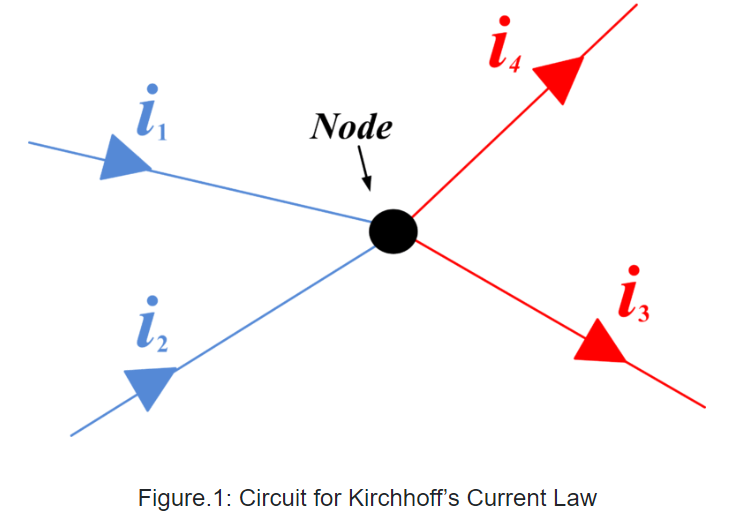
\includegraphics[width=0.3\textwidth]{pic1.png}
\end{wrapfigure}
The algebraic sum of currents in a network of conductors meeting at a point is zero, or the sum of currents entering into any node (junction) in an electrical circuit is equal to the amount of currents flowing out of that node. This legislation is built on the principle of charge conservation. The net current is 0 at the darkest point, for example, meaning that:
\begin{equation}
    i_{1} + i_{2} = i_{3} + i_{4}
\end{equation}

\subsubsection{Kirchhoff's Voltage Law}
\begin{wrapfigure}{R}{0.2\textwidth}
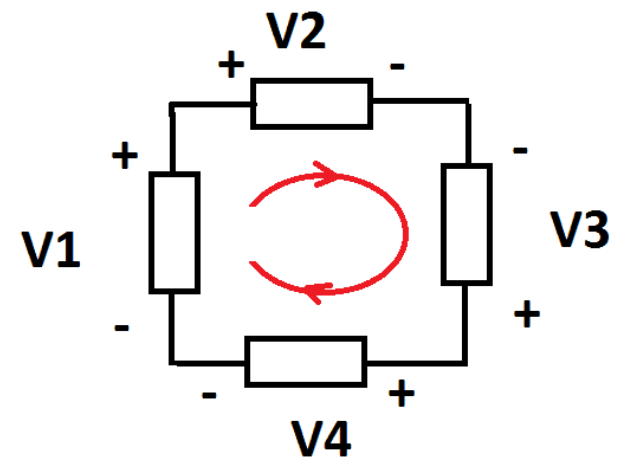
\includegraphics[width=0.3\textwidth]{pic2.png}
\end{wrapfigure}
The directed sum of the electrical potential difference (voltage) around any closed network is zero; or, to put it another way, the algebraic sum of the resistances and currents of the conductors in a closed loop equals the total emf available in that loop. As illustrated by this equation, the total of all voltages encircling a loop is zero.
\begin{equation}
    \Sigma V_{i} = 0
\end{equation}
\newpage
\subsection{Circuit Setup}
\subsubsection{Circuit Diagram}
\begin{center}
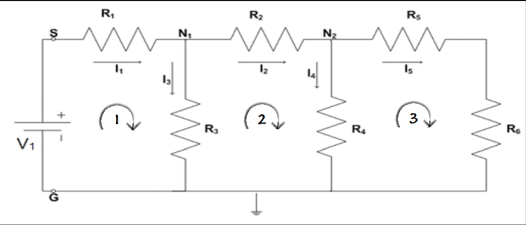
\includegraphics[width=1\textwidth]{pic3.png}    
\end{center}
Here, $V_1$ = 5V, $R_1$ = $R_2$ = 100\si{\ohm}, $R_3$ = $R_4$ = 220\si{\ohm}, $R_5$ = 47\si{\ohm}, $R_6$ = 150\si{\ohm}
\subsubsection{Combined Circuit}
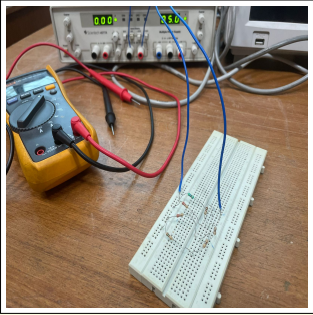
\includegraphics[width=0.5\textwidth]{pic5.png}
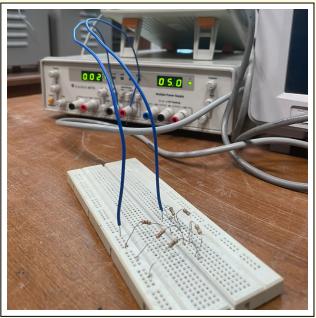
\includegraphics[width=0.5\textwidth]{pic4.png}

\subsection{Observations}
\begin{tabular}{|c|c|c|}
\hline
    Resistors(in \si{\ohm}) & Measured Voltage(in V) & Calculated Current(in mA) \\
    \hline
    $R_1$=100\si{\ohm} & 2.47 & 24.7 \\
    $R_2$=100\si{\ohm} & 1.27 & 12.7 \\
    $R_3$=220\si{\ohm} & 2.58 & 11.7 \\
    $R_4$=220\si{\ohm} & 1.31 & 5.95 \\
    $R_5$=47\si{\ohm} & 0.31 & 6.59 \\
    $R_6$=150\si{\ohm} & 1.00 & 6.66 \\
\hline
\end{tabular}
\subsection{Verification of Kirchhoff's Current Law}
\subsubsection{Node 1}
Incoming Current: $i_1$ = 24.7 mA \\
Outgoing Current: $i_2$+$i_3$ = 12.7mA + 11.7mA = 24.4mA =  Incoming Current. \\
As Incoming Current is approximately equal to Outgoing Current, Kirchhoff’s Current Law is verified.

\subsubsection{Node 2}
Note: $i_5$ = $i_6$, thus we take $i_5$ as the average of obtained values of $i_5$ and $i_6$. \\
Thus, $i_5$ = $i_6$ = 6.63mA \\
\\
Incoming Current: i2 = 12.7mA \\
Outgoing Current: i4+i5 = 5.95mA + 6.63mA = 12.58mA = Incoming Current. \\
As Incoming Current is approximately equal to Outgoing Current, Kirchhoff’s Current Law is verified.
\subsection{Verification of Kirchhoff ’s Current Law}
\subsubsection{Loop 1}
Potential Drop: $V_1$ - $V_{R_1}$ - V = 5V - 2.47V - 2.58V = -0.05V \approx 0V \\
As Potential Drop is approx. equal to 0, Kirchhoff’s Voltage Law is verified.
\subsubsection{Loop 2}
Potential Drop: $V_{R_3}$ - $V_{R_2}$ - $V_{R_4}$ = 2.58V - 1.27V - 1.31V = 0V \approx 0V \\
As Potential Drop is approximately equal to 0, Kirchhoff’s Voltage Law is verified.
\subsubsection{Loop 3}
Potential Drop: $V_{R_4}$ − $V_{R_5}$ − $V_{R_6}$ = 1.31V - 1V - 0.31V = 0V \approx 0V \\
As Potential Drop is approximately equal to 0, Kirchhoff’s Voltage Law is verified.

\subsection{Change in $i_5$ when $R_7$ = 470$\Omega$ is connected across SG}
$V_5$' = 0.309V\\
\therefore Thus, there is negligible change in $i_5$. \\
The variation in the reading may be due to some finite resistance in the connecting
wires.
\end{document}
